\documentclass{beamer}
\usepackage{amsmath, amssymb, graphicx}
\usepackage{bm} % For bold math symbols

\usetheme{Madrid}

\title{Principal Component Analysis}
\author{Naman Pesricha}
\date{\today}

\begin{document}

\begin{frame}
    \titlepage
\end{frame}

% Slide 1: Notations
\begin{frame}{Notations}
    \begin{itemize}
        \item $\mathbf{X} \in \mathbb{R}^{n \times d}$: Mean-centered data matrix with $n$ samples and $d$ features
        \item $ \mathbf{X}^\top\mathbf{X}$: Covariance matrix (symmetric positive semi-definite)
        \item $\mathbf{\Lambda} = \text{diag}(\lambda_1, \ldots, \lambda_d)$: Diagonal eigenvalue matrix
        \item $\mathbf{U}, \mathbf{\Sigma}, \mathbf{V}$: SVD components where $\mathbf{X} = \mathbf{U}\mathbf{\Sigma}\mathbf{V}^\top$
        \item $\sigma_i$: Singular values 
        \item $\|\cdot\|_F$: Frobenius norm; $\|\cdot\|_2$: 2 norm
        \item $\kappa(\mathbf{X})$: Condition number of matrix $\mathbf{X}$
        \item $\mathcal{L}(\mathbf{v}, \alpha, \mu)$: Lagrangian function with multiplier $\alpha$ and $\mu$
        \item $\nabla f$ denotes the gradient, and $\nabla_{\mathbf{x}} f$ is the gradient with respect to $\mathbf{x}$.
        \item $n_{\text{samples}}$ or $n$: Number of data samples
        \item $n_{\text{features}}$ or $d$: Number of features/dimensions
        \item $n_{\text{components}}$ or $k$: Number of principal components to keep
    \end{itemize}
\end{frame}

\begin{frame}{What is PCA?}
    \begin{block}{Principal Component Analysis }
    \begin{itemize}
        \item Principal component analysis (PCA) is a linear dimensionality reduction technique with applications in exploratory data analysis, visualization and data preprocessing.
        
        \item The data is linearly transformed onto a new coordinate system such that the directions (principal components) capturing the largest variation in the data can be easily identified.
        
    \end{itemize}
        
    \end{block}

    \begin{itemize}
    \item \textbf{Principal Directions}: Orthogonal vectors that define the directions of maximum variance in the original feature space (New orthonormal basis vectors).
    \item \textbf{Principal Components}: Coordinates of the data projected onto the principal directions; they represent the data in the new rotated basis.
    \end{itemize}

    
    \footnotesize{Source: \scriptsize{https://en.wikipedia.org/wiki/Principal\_component\_analysis}}
\end{frame}

\begin{frame}{Applications of Principal Component Analysis}
    \vspace{0.5cm}
    
    \large\textbf{Dimensionality Reduction for Machine Learning}\\
    Reduces feature space while preserving variance, improving model training speed and performance.\\
    
    \vspace{0.5cm}
    
    \large\textbf{Exploratory Data Visualization}\\
    Projects high-dimensional datasets to 2D/3D for intuitive pattern recognition and cluster analysis.\\
    
    \vspace{0.5cm}
    
    \large\textbf{Signal Processing and Noise Reduction}\\
    Isolates dominant signal components while filtering out noise in time-series and image data.\\
    
\end{frame}

\begin{frame}{Mathematical Foundations: \textbf{\underline{Symmetric}} Positive Definite Matrices and KKT Conditions}

\begin{block}{Properties of Symmetric Matrices}
    Let $\bm{A} \in \mathbb{R}^{n \times n}$ be a symmetric matrix ($\bm{A} = \bm{A}^{\top}$).
    
    \begin{itemize}
        \item $\bm{A} = \bm{A}^{\top}$ (by definition of symmetry)
        \item All eigenvalues of $\bm{A}$ are real
        \item Eigenvectors of symmetric matrices can be chosen to form an orthogonal set
    \end{itemize}
\end{block}

\vspace{0.3cm}

\textbf{Proof: Eigenvalues of $\bm{A}$ are real}  

Let $\lambda \in \mathbb{C}$ and $\bm{v} \in \mathbb{C}^n$ be an eigenpair:
\[
\bm{A}\bm{v} = \lambda \bm{v}, \quad \bm{v} \neq \bm{0}
\]
Consider $\bm{v}^* \bm{A} \bm{v}$:
\[
\bm{v}^* \bm{A} \bm{v} = \bm{v}^* (\lambda \bm{v}) = \lambda \bm{v}^* \bm{v}
\]

\end{frame}

\begin{frame}{Mathematical Foundations: \textbf{\underline{Symmetric}} Positive Definite Matrices and KKT Conditions}

Taking conjugate transpose of $\bm{A}\bm{v} = \lambda \bm{v}$:
\[
(\bm{A}\bm{v})^* = (\lambda \bm{v})^* \quad \Rightarrow \quad \bm{v}^* \bm{A} = \bar{\lambda} \bm{v}^*
\]
Thus:
\[
\bm{v}^* \bm{A} \bm{v} = \bar{\lambda} \bm{v}^* \bm{v}
\]
Equating both expressions:
\[
\lambda \bm{v}^* \bm{v} = \bar{\lambda} \bm{v}^* \bm{v}
\]
Since $\bm{v}^* \bm{v} > 0$, we get $\boxed{\lambda = \bar{\lambda} \quad \Rightarrow \quad \lambda \in \mathbb{R}}$


\end{frame}

\begin{frame}{Mathematical Foundations: \textbf{\underline{Symmetric}} Positive Definite Matrices and KKT Conditions}

\textbf{Proof: Eigenvectors of symmetric matrices can be chosen to form an orthogonal set}

Let $\bm{A} \in \mathbb{R}^{n \times n}$ be symmetric and let $\lambda_1 \neq \lambda_2$ with corresponding eigenvectors $\bm{v}_1$ and $\bm{v}_2$.

We have:
\[
\bm{A}\bm{v}_1 = \lambda_1 \bm{v}_1, \quad \bm{A}\bm{v}_2 = \lambda_2 \bm{v}_2
\]
Consider:
\[
\bm{v}_2^{\top} \bm{A} \bm{v}_1 = \bm{v}_2^{\top} (\lambda_1 \bm{v}_1) = \lambda_1 \bm{v}_2^{\top} \bm{v}_1
\]
Using symmetry ($\bm{A} = \bm{A}^{\top}$):
\[
\bm{v}_2^{\top} \bm{A} \bm{v}_1 = (\bm{A} \bm{v}_2)^{\top} \bm{v}_1 = (\lambda_2 \bm{v}_2)^{\top} \bm{v}_1 = \lambda_2 \bm{v}_2^{\top} \bm{v}_1
\]

\end{frame}

\begin{frame}{Mathematical Foundations: \textbf{\underline{Symmetric}} Positive Definite Matrices and KKT Conditions}

Thus:
\[
\lambda_1 \bm{v}_2^{\top} \bm{v}_1 = \lambda_2 \bm{v}_2^{\top} \bm{v}_1
\]
Since $\lambda_1 \neq \lambda_2$, we conclude:
\[
\boxed{\bm{v}_2^{\top} \bm{v}_1 = 0 \quad \Rightarrow \quad \bm{v}_1 \perp \bm{v}_2}
\]

If some eigenvalues are repeated, we can still choose orthogonal eigenvectors within the corresponding eigenspace. These are also orthogonal to eigenvectors of distinct eigenvalues. The proof for this is beyond the scope of this course. Interested students can contact the TAs.
\vspace{0.3cm}
Thus, the proof is complete.

\end{frame}

\begin{frame}{Mathematical Foundation: \textbf{\underline{Symmetric Positive Definite}} Matrices and KKT Conditions}

\begin{block}{Definition: Symmetric Positive Definite (PD) Matrix}

A symmetric matrix $\bm{A} \in \mathbb{R}^{n \times n}$ is \textbf{positive definite} if:
\[
\bm{A} = \bm{A}^\top \quad \text{and} \quad \bm{v}^\top \bm{A} \bm{v} > 0 \quad \forall \, \bm{v} \in \mathbb{R}^n, \, \bm{v} \neq \bm{0}
\]

If $\bm{v}^\top \bm{A} \bm{v} \geq 0$ for all $\bm{v} \neq \bm{0}$, then $\bm{A}$ is \textbf{positive semi-definite (PSD)}.

\vspace{0.3cm}

\textbf{Key properties:}
\begin{itemize}
    \item $\bm{A} = \bm{A}^\top$ (symmetric)
    \item $\bm{v}^\top \bm{A} \bm{v} > 0$ for all $\bm{v} \neq \bm{0}$
    \item All eigenvalues are real $\lambda_i > 0$ $\forall i$
    \item Eigenvectors of PD matrices can be chosen to form an orthogonal set
\end{itemize}

\end{block}

\end{frame}

\begin{frame}{Mathematical Foundation: \textbf{\underline{Symmetric Positive Definite}} Matrices and KKT Conditions}

\textbf{Proof: For a symmetric positive definite matrix, all eigenvalues are positive}

Let $\lambda$ be an eigenvalue with eigenvector $\bm{v} \neq \bm{0}$:
\[
\bm{A} \bm{v} = \lambda \bm{v}
\]
Consider:
\[
\bm{v}^\top \bm{A} \bm{v} = \bm{v}^\top (\lambda \bm{v}) = \lambda \bm{v}^\top \bm{v}
\]
Since $\bm{v}^\top \bm{v} > 0$ and $\bm{v}^\top \bm{A} \bm{v} > 0$, it follows:
\[
\lambda \bm{v}^\top \bm{v} > 0 \quad \Rightarrow \quad \lambda > 0
\]
Thus:
\[
\boxed{\lambda_i > 0 \quad \forall \, i = 1,2,\dots, n}
\]

\end{frame}


\begin{frame}{Mathematical Foundation: \textbf{\underline{Symmetric Positive Definite}} Matrices and KKT Conditions}

\begin{block}{Definition: Symmetric Positive Semi-Definite (PSD) Matrix}

A symmetric matrix $\bm{A} \in \mathbb{R}^{n \times n}$ is \textbf{positive semi-definite} if:
\[
\bm{A} = \bm{A}^\top \quad \text{and} \quad \bm{v}^\top \bm{A} \bm{v} \geq 0 \quad \forall \, \bm{v} \in \mathbb{R}^n, \, \bm{v} \neq \bm{0}
\]

\vspace{0.3cm}

\textbf{Key properties:}
\begin{itemize}
    \item $\bm{A} = \bm{A}^\top$ (symmetric)
    \item $\bm{v}^\top \bm{A} \bm{v} \geq 0$ for all $\bm{v} \neq \bm{0}$
    \item All eigenvalues are real $\lambda_i \geq 0$ $\forall i$
    \item Eigenvectors can be chosen to form an orthogonal set
\end{itemize}

\end{block}

\end{frame}

\begin{frame}{Mathematical Foundation: \textbf{\underline{Symmetric Positive Definite}} Matrices and KKT Conditions}

\begin{alertblock}{Comparison: PD vs PSD Matrices}

\begin{tabular}{ll}
\textbf{PD} & \textbf{PSD} \\
\hline
\hfill \\
$\bm{v}^\top \bm{A} \bm{v} > 0$ & $\bm{v}^\top \bm{A} \bm{v} \geq 0$ \\
$\lambda_i > 0$ & $\lambda_i \geq 0$ \\
Invertible & May be singular \\
$\det(\bm{A}) > 0$ & $\det(\bm{A}) \geq 0$ \\
Strictly convex quadratic form & Convex quadratic form \\
\end{tabular}

\vspace{0.3cm}

Note: Every PD matrix is PSD, but not conversely.

\end{alertblock}

\end{frame}

% BEGIN KKT

\begin{frame}{{Mathematical Foundation: Symmetric Positive Definite Matrices and \textbf{\underline{KKT Conditions}}}}

    Karush-Kuhn-Tucker (KKT) conditions provide a mathematical framework for identifying optimal solutions to constrained optimization problems.
    
    \begin{itemize}
        \item Capture both objective and constraint behavior through gradient conditions.
        \item Identify which constraints are active at the optimal point.
        \item Help \textbf{verification} of optimality in general problems and \textbf{certification} in convex problems.
    \end{itemize}

\end{frame}


\begin{frame}{{Mathematical Foundation: Symmetric Positive Definite Matrices and \textbf{\underline{KKT Conditions}}}}

    \textbf{1. Verification (General / Non-Convex Case)}
    \begin{itemize}
        \item KKT conditions are \textbf{necessary but not sufficient}.
        \item A point satisfying KKT is a \textbf{candidate} for optimality (optima or saddle point)
        \item Must verify using second-order conditions or objective comparison.
        \item \textit{Think of KKT as a filter — not a final verdict.}
    \end{itemize}
    
    \medskip
    
    \textbf{2. Certification (Convex Case)}
    \begin{itemize}
        \item KKT conditions are \textbf{necessary and sufficient}.
        \item If a point satisfies KKT, it is \textbf{guaranteed to be globally optimal}.
        \item Requires convex problem (convex $f$, convex $g_j$, affine $h_k$. Subsequent slides will give more clarity).
        \item \textit{Think of KKT as both filter and proof.}
    \end{itemize}

\end{frame}


\begin{frame}{{Mathematical Foundation: Symmetric Positive Definite Matrices and \textbf{\underline{KKT Conditions}}}}
    \begin{block}{Problem Setup: General Constrained Optimization Problem}
        \[
            \text{Min } f(\bm{x}) \quad \text{s.t.} \quad
            \begin{cases}
                g_j(\bm{x}) \leq 0 & j = 1,\ldots,J \\
                h_k(\bm{x}) = 0 & k = 1,\ldots,K
            \end{cases}
        \]

        \begin{itemize}
            \item \textbf{Decision variables}: $\bm{x} \in \mathbb{R}^n$
            \item \textbf{Objective}: $f: \mathbb{R}^n \rightarrow \mathbb{R}$
            \item \textbf{Feasible set}: $\{\bm{x} | g_j(\bm{x}) \leq 0, h_k(\bm{x}) = 0\}$
        \end{itemize}
    \end{block}

    \textbf{Constraint Classification}
    \begin{itemize}
    \item \textbf{ACTIVE}: Constraints satisfied exactly at $\mathbf{x^*}$ ($g_i(\mathbf{x^*}) = 0$)
    \begin{itemize}
        \item Can be violated by an infinitesimal step in a non-feasible direction
    \end{itemize}
    
    \item \textbf{INACTIVE}: Constraints satisfied with slack at $\mathbf{x^*}$ ($g_i(\mathbf{x^*}) < 0$)
    \begin{itemize}
        \item Remain satisfied for all infinitesimal steps around $x^*$
    \end{itemize}
\end{itemize}
\end{frame}

\begin{frame}{{Mathematical Foundation: Symmetric Positive Definite Matrices and \textbf{\underline{KKT Conditions}}}}
    \begin{block}{Constraint Sets}
        For feasible $\bm{x}^*$:
        \begin{itemize}
            \item \textbf{Active constraints} ($Ac$):
                \begin{itemize}
                    \item Inequalities: $Ac_I = \{j \mid g_j(\bm{x}^*) = 0\}$
                    \item Equalities: $Ac_E = \{1,\ldots,K\}$ (always active)
                \end{itemize}

            \item \textbf{Inactive constraints} ($Ic$):
                \begin{itemize}
                    \item Inequalities: $Ic = \{j \mid g_j(\bm{x}^*) < 0\}$
                \end{itemize}
        \end{itemize}
    \end{block}

    \begin{block}{Regularity Condition}
        $\bm{x}^*$ is \textbf{regular} iff:
        \[
            \mathrm{rank}\left(\{\nabla g_j(\bm{x}^*)\}_{j \in Ac_I} \cup \{\nabla h_k(\bm{x}^*)\}_{k \in Ac_E}\right) = |Ac_I| + |Ac_E|
        \]
        i.e., the active constraint gradients are linearly independent.
    \end{block}
\end{frame}

\begin{frame}{{Mathematical Foundation: Symmetric Positive Definite Matrices and \textbf{\underline{KKT Conditions}}}}
    \begin{block}{Lagrangian Function}
        \[
            \mathcal{L}(\bm{x}, \bm{\mu}, \bm{\alpha}) = f(\bm{x}) 
            + \underbrace{\sum_{j=1}^J \mu_j g_j(\bm{x})}_{\text{inequalities}} 
            + \underbrace{\sum_{k=1}^K \alpha_k h_k(\bm{x})}_{\text{equalities}}
        \]
        \begin{itemize}
            \item $\alpha_k \in \mathbb{R}$: Equality multipliers
            \item $\mu_j \geq 0$: Inequality multipliers
        \end{itemize}
    \end{block}
\end{frame}

\begin{frame}{{Mathematical Foundation: Symmetric Positive Definite Matrices and \textbf{\underline{KKT Conditions}}}}
    \begin{block}{KKT Conditions Part I}
        For \textbf{regular} local minimum $\bm{x}^*$:

        1. \textbf{Stationarity}:
        Derivative wrt $\bm{x}$ is 0 at $\bm{x}$ = $\bm{x}^*$.
        \[
            \nabla_{\bm{x}} \mathcal{L}(\bm{x}^*, \bm{\mu}, \bm{\alpha}) = \bm{0}
        \]
        \[
            \Rightarrow \nabla f(\bm{x}^*) + \sum_{j=1}^J \mu_j \nabla g_j(\bm{x}^*) + \sum_{k=1}^K \alpha_k \nabla h_k(\bm{x}^*) = \bm{0}
        \]

        2. \textbf{Primal Feasibility}:
        All constraints should be satisfied at $\bm{x^*}$.
        \[
            g_j(\bm{x}^*) \leq 0 \quad \forall j, \quad h_k(\bm{x}^*) = 0 \quad \forall k
        \]
    \end{block}
\end{frame}

\begin{frame}{{Mathematical Foundation: Symmetric Positive Definite Matrices and \textbf{\underline{KKT Conditions}}}}
    \begin{block}{KKT Conditions Part II}
        3. \textbf{Dual Feasibility}: 
        Dual feasibility ($\mu_j \geq 0$) ensures the gradient balance $\nabla f = -\sum \mu_j \nabla g_j$ opposes constraint violations.
        \[
            \mu_j \geq 0 \quad \forall j = 1,\ldots,J
        \]

        4. \textbf{Complementary Slackness}:
        \[
            \mu_j g_j(\bm{x}^*) = 0 \quad \forall j
        \]
        \begin{itemize}
            \item Implies $\mu_j = 0$ for inactive constraints
            \item Active constraints may have $\mu_j > 0$
        \end{itemize}
    \end{block}
\end{frame}

\begin{frame}{{Mathematical Foundation: Symmetric Positive Definite Matrices and \textbf{\underline{KKT Conditions}}}}

    \framebox{\parbox{\linewidth}{
        \textbf{Goal:} Given a point \(\mathbf{x^*}\), verify whether it satisfies 
        the necessary \\ conditions for optimality.
    }}

    \medskip

    \textbf{What we do:}
    \begin{itemize}
        \item Check that \(\mathbf{x^*}\) is a \textbf{regular point} (i.e., constraint qualification holds).
        \item Evaluate whether the KKT conditions are satisfied at point \(\mathbf{x^*}\).
    \end{itemize}
    
    \textbf{Interpretation of Results:}
    \begin{itemize}
        \item If KKT conditions are \textbf{not satisfied}, then:
        \begin{itemize}
            \item \(\mathbf{x^*}\) is \textbf{not optimal} (fails necessary conditions).
        \end{itemize}
        \item If KKT conditions \textbf{are satisfied}, then:
        \begin{itemize}
            \item In a \textbf{convex problem} → \(\mathbf{x^*}\) is \textbf{globally optimal}.
            \item In a \textbf{non-convex problem} → \(\mathbf{x^*}\) is a \textbf{candidate only}; further analysis (e.g., second-order conditions, objective comparison) is required.
        \end{itemize}
    \end{itemize}

    \textit{KKT verification is a checkpoint — necessary but not always conclusive.}
    
\end{frame}

\begin{frame}{{Mathematical Foundation: Symmetric Positive Definite Matrices and \textbf{\underline{KKT Conditions}}}}
    \begin{block}{KKT: Takeaways}
        \begin{itemize}
            \item KKT conditions are \textbf{necessary} for local optimality at \textbf{regular} points
            \item Regularity requires linear independence of active constraint gradients
            \item For convex problems (convex $f$, convex $g_j$, affine $h_k$), KKT becomes \textbf{sufficient}
            \item In convex cases, KKT solutions are \textbf{global minima}
            \item Complementary slackness reveals which constraints are active ($\mu_j > 0$ for active and $\mu_j = 0$ for inactive)
        \end{itemize}
    \end{block}

    \begin{alertblock}{Key Insight}
        KKT serves as both optimality \textbf{verification} (necessary in non-convex) and \textbf{certification} (sufficient in convex cases)
    \end{alertblock}
\end{frame}

% END KKT

\begin{frame}{PCA: Two Interpretations}
    \begin{block}{Principal Component Analysis}
        Let $\mathbf{X}$ be the $n \times d$ mean-centered data matrix ($n$ samples, $d$ features):
        
        \begin{enumerate}
            \item \textbf{Maximum Variance Interpretation}:
            The 1st PC is a unit vector $\mathbf{v}_1$ maximizing variance of projections:
            \[
             \mathbf{v}_1 = \underset{\|\mathbf{v}\|=1}{\arg\max} \sum_{i = 1}^n (\mathbf{v}^\top \mathbf{x_i})^2 =  \underset{\|\mathbf{v}\|=1}{\arg\max} \|\mathbf{X}\mathbf{v}\|^2 = \underset{\|\mathbf{v}\|=1}{\arg\max}\ \mathbf{v}^\top (\mathbf{X}^\top \mathbf{X}) \mathbf{v}
            \]
            
            \item \textbf{Minimum Reconstruction Interpretation}:
            The 1st PC minimizes reconstruction error for all samples:
            \[
            \mathbf{v}_1 = \underset{\|\mathbf{v}\|=1}{\arg\min} \sum_{i=1}^n \|\mathbf{x}_i - (\mathbf{x}_i^\top \mathbf{v})\mathbf{v}\|_2^2
            \]
        \end{enumerate}
    \end{block}
\end{frame}

\begin{frame}{Equivalence of PCA Interpretations}
        For mean-centered $\mathbf{X} \in \mathbb{R}^{n \times d}$ and $\|\mathbf{v}\|_2 = 1$:
        \begin{align*}
            &\text{\textbf{Min-Recon}}: \quad \min_{\|\mathbf{v}\|=1} \sum_{i=1}^n \|\mathbf{x}_i - (\mathbf{x}_i^\top \mathbf{v})\mathbf{v}\|_2^2 \\
            &= \min_{\|\mathbf{v}\|=1} \sum_{i=1}^n \left( \|\mathbf{x}_i\|_2^2 - (\mathbf{x}_i^\top \mathbf{v})^2 \right) \\
            &= C - \max_{\|\mathbf{v}\|=1} \sum_{i=1}^n (\mathbf{x}_i^\top \mathbf{v})^2 \\
            &= C - \max_{\|\mathbf{v}\|=1} \|\mathbf{X}\mathbf{v}\|_2^2 \quad \text{\textbf{(Max-Var)}} 
        \end{align*}
        where $C = \sum_{i=1}^n \|\mathbf{x}_i\|_2^2$ is data-dependent but constant w.r.t $\mathbf{v}$.

\end{frame}

%FIRST INTER

\begin{frame}{Maximum Variance Interpretation}

We will show how to get the first principal component $\mathbf{v_1}$ from Maximum Variance Interpretation. The other interpretation is not covered, and is to be considered a non evaluated homework.

\vspace{0.3cm}

    \begin{block}{Problem Formulation}
        Given mean-centered data $\mathbf{X} \in \mathbb{R}^{n \times d}$:
        \vspace{-0.2cm}
        \[
        \underset{\mathbf{v}}{\text{maximize}}\ \mathbf{v}^\top \mathbf{X}^\top \mathbf{X} \mathbf{v} \quad \text{subject to}\quad \mathbf{v}^\top \mathbf{v} = 1
        \]
        \begin{itemize}
            \item $\mathbf{X}^\top \mathbf{X}$ = $d \times d$ covariance matrix
            \item $\mathbf{v}$ = unit direction vector (principal direction)
        \end{itemize}
    \end{block}
\end{frame}

\begin{frame}{Maximum Variance Interpretation}
    \begin{block}{Equivalent Minimization Problem}
        Convert to standard minimization form:
        \[
        \underset{\mathbf{v}}{\text{minimize}}\ -\mathbf{v}^\top \mathbf{X}^\top \mathbf{X} \mathbf{v} \quad \text{s.t.}\quad \mathbf{v}^\top \mathbf{v} - 1 = 0
        \]
        \begin{itemize}
            \item Same solution since $\text{max}\ f = \text{min}\ -f$
            \item Now compatible with standard KKT framework
        \end{itemize}
    \end{block}
\end{frame}

\begin{frame}{Maximum Variance Interpretation}
    \begin{block}{Lagrangian Formulation}
        Introduce Lagrange multiplier $\alpha$ for the equality constraint:
        \[
        \mathcal{L}(\mathbf{v}, \alpha) = -\mathbf{v}^\top \mathbf{X}^\top \mathbf{X} \mathbf{v} + \alpha(\mathbf{v}^\top \mathbf{v} - 1)
        \]
        \begin{itemize}
            \item First term: Objective function
            \item Second term: Constraint with multiplier
        \end{itemize}
    \end{block}
\end{frame}

\begin{frame}{Maximum Variance Interpretation}
    \begin{block}{KKT Stationarity Condition}
        Take derivative w.r.t $\mathbf{v}$ and set to zero:
        \[
        \nabla_{\mathbf{v}} \mathcal{L} = -2\mathbf{X}^\top \mathbf{X} \mathbf{v} + 2\alpha \mathbf{v} = \mathbf{0}
        \]
        Simplifies to the eigenvalue problem:
        \[
        \mathbf{X}^\top \mathbf{X} \mathbf{v} = \alpha \mathbf{v}
        \]
    Note that $\alpha$ is an eigenvalue of the covariance like matrix $ \mathbf{X}^\top \mathbf{X}$ with eigenvector $\mathbf{v}$. 
    \end{block}
\end{frame}

\begin{frame}{Maximum Variance Interpretation}
    \begin{block}{Objective Value at Critical Point}
        Substitute $\mathbf{X}^\top \mathbf{X} \mathbf{v} = \alpha \mathbf{v}$ back:
        \[
        -\mathbf{v}^\top \mathbf{X}^\top \mathbf{X} \mathbf{v} = -\mathbf{v}^\top (\alpha \mathbf{v}) = -\alpha \underbrace{\mathbf{v}^\top \mathbf{v}}_{=1} = -\alpha
        \]
        \begin{itemize}
            \item To minimize $-\alpha$, we must maximize $\alpha$
            \item Thus seek the largest eigenvalue $\alpha$
            \item Since $ \mathbf{X}^\top \mathbf{X} \in \mathbb{R}^{d\times d}$ is a PSD matrix, 
            \[
            \lambda_1 \geq \lambda_2 \geq \cdots \geq \lambda_d \geq0
            \]
        \end{itemize}
    \end{block}
\end{frame}

\begin{frame}{Maximum Variance Interpretation}
    \begin{alertblock}{Optimal Solution}
        The principal component is the eigenvector $\mathbf{v}_1$ corresponding to:
        \[
        \alpha_{\text{max}} = \lambda_1 \quad \text{(Largest eigenvalue)}
        \]
        \begin{itemize}
            \item Captured variance: $\mathbf{v}_1^\top \mathbf{X}^\top \mathbf{X} \mathbf{v}_1 = \lambda_1$
            \item Subsequent components: Eigenvectors of next largest eigenvalues
        \end{itemize}
    \end{alertblock}
\end{frame}

\begin{frame}{Maximum Variance Interpretation}
    \begin{block}{Sequential Components}
        For $k^{th}$ component ($k > 1$):
        \[
        \tilde{\mathbf{X}}_k = \mathbf{X} - \mathbf{X}\sum_{i=1}^{k-1}\mathbf{v}_i\mathbf{v}_i^\top
        \]
        \begin{itemize}
            \item Remove variance explained by previous components
            \item Solve same optimization for $\tilde{\mathbf{X}}_k$
            \item Yields orthogonal eigenvectors $\mathbf{v}_1, \mathbf{v}_2, ...$
        \end{itemize}
    \end{block}
\end{frame}


\begin{frame}{Maximum Variance Interpretation}
    \begin{block}{Variance Capture Ratio}
        The $k^{th}$ principal component captures:
        \[
        \text{Variance ratio} = \frac{\lambda_k}{\sum_{i=1}^d \lambda_i}
        \]
        where $\lambda_i$ are eigenvalues of $\mathbf{X}^\top \mathbf{X}$ such that $
            \lambda_1 \geq \lambda_2 \geq \cdots \geq \lambda_d \geq0
            $.
    \end{block}

    \textbf{Practical Implications}
        \begin{itemize}
            \item First PC typically captures 60-90\% of total variance
            \item Common threshold: Keep components covering $\geq$ 95\% cumulative variance. If \#components = $k$
            \[
            \boxed{\text{Cumulative Explained Variance = }\frac{\sum_{i=1}^k \lambda_i}{\sum_{i=1}^d \lambda_i} \geq 0.95}
            \]
            \item Example: 100D data $\rightarrow$ might need only 5-10 PCs
        \end{itemize}

\end{frame}


%END FIRST INTER


\begin{frame}{Sklearn PCA}

The \texttt{sklearn}'s PCA\footnote{\scriptsize{https://scikit-learn.org/stable/modules/generated/sklearn.decomposition.PCA.html}} uses three major algorithms for computing PCA:
\begin{enumerate}
    \item \textbf{Eigenvalue Decomposition} 
    \begin{itemize}
        \item Used when \( n_{\text{features}} < 1000 \) \textbf{and} \( n_{\text{samples}} > 10 \times n_{\text{features}} \).
        \item Best for small \( n_{\text{features}} \) and \( n_{\text{samples}} \gg n_{\text{features}} \).
        \item Doubles the condition number \( \kappa \) and hence worst for ill conditioned covariance matrices.
        \item Less numerically stable than full SVD.
    \end{itemize}

    \item \textbf{Randomized SVD} 
    \begin{itemize}
        \item Used when data is larger than \( 500 \times 500 \) \textbf{and} \( n_{\text{components}} < 80\% \) of \( \min(n_{\text{samples}}, n_{\text{features}}) \).
        \item Faster than full SVD under these conditions.
        \item Lower memory footprint compared to full SVD.
    \end{itemize}

    \item \textbf{Full SVD} 
    \begin{itemize}
        \item Default fallback when no other conditions apply.
        \item High time complexity.
        \item Large memory footprint.
    \end{itemize}
\end{enumerate}

\end{frame}


% Decomp

\begin{frame}{General Eigenvalue Decomposition}
    \begin{block}{EVD for Non-Defective Matrices}
        For any square matrix $\mathbf{A} \in \mathbb{R}^{d \times d}$:
        \[
        \mathbf{A} = \mathbf{V}\mathbf{\Lambda}\mathbf{V}^{-1}
        \]
        \begin{itemize}
            \item \textbf{Existence Condition}:
            \begin{itemize}
                \item Requires $\mathbf{A}$ to be non-defective
                \item Matrix is non-defective if the set of eigenvectors is linearly independent.
            \end{itemize}
            \item $\mathbf{V}$ contains eigenvectors (may not be orthogonal)
            \item $\mathbf{\Lambda}$ diagonal with eigenvalues
        \end{itemize}
    \end{block}
\end{frame}

\begin{frame}{EVD for PCA (Spectral Decomposition)}
    \begin{block}{EVD Special Case: Symmetric Matrices}
        For mean-centered data $\mathbf{X} \in \mathbb{R}^{n \times d}$ and symmetric $\mathbf{A} = \mathbf{X}^\top\mathbf{X}$:
        \[
        \mathbf{A} = \mathbf{V}\mathbf{\Lambda}\mathbf{V}^\top
        \]
        \begin{itemize}
            \item \textbf{Guaranteed Properties}:
            \begin{itemize}
                \item Always exists (symmetric matrices are non-defective)
                \item $\mathbf{V}$ is orthogonal ($\mathbf{V}^{-1} = \mathbf{V}^\top$)
                \item All eigenvalues real and non-negative
            \end{itemize}
            \item $\mathbf{V} = [\mathbf{v}_1 \cdots \mathbf{v}_d]$ contains orthonormal eigenvectors (columns are principal directions)
            \item $\mathbf{\Lambda} = \text{diag}(\lambda_1, \ldots, \lambda_d)$ with $\lambda_1 \geq \cdots \geq \lambda_d \geq 0$
        \end{itemize}
    \end{block}
\end{frame}

\begin{frame}{SVD for PCA}
    \begin{block}{Singular Value Decomposition}
        For mean-centered data $\mathbf{X} \in \mathbb{R}^{n \times d}$:
        \[
        \mathbf{X} = \mathbf{U}\mathbf{\Sigma}\mathbf{V}^\top
        \]
        \begin{itemize}
            \item \textbf{Universal existence}: For any real/complex matrix
            \item $\mathbf{U} \in \mathbb{R}^{n \times n}$, $\mathbf{V} \in \mathbb{R}^{d \times d}$ orthogonal (columns are principal directions)
            \item $\mathbf{\Sigma} = \begin{pmatrix}
                \text{diag}(\sigma_1, \ldots, \sigma_r) & \mathbf{0} \\
                \mathbf{0} & \mathbf{0}
            \end{pmatrix}$, $r = \text{rank}(\mathbf{X})$
            \item $\sigma_i = \sqrt{\lambda_i}$ where $\lambda_i$ are eigenvalues of $\mathbf{X}^\top\mathbf{X}$
        \end{itemize}
    \end{block}
\end{frame}

% END DECOMP


% EXAMPLES

\begin{frame}{Exploratory Data Visualization}
    \begin{center}
        \scriptsize{4D iris dataset data project to PC1 and PC2}
        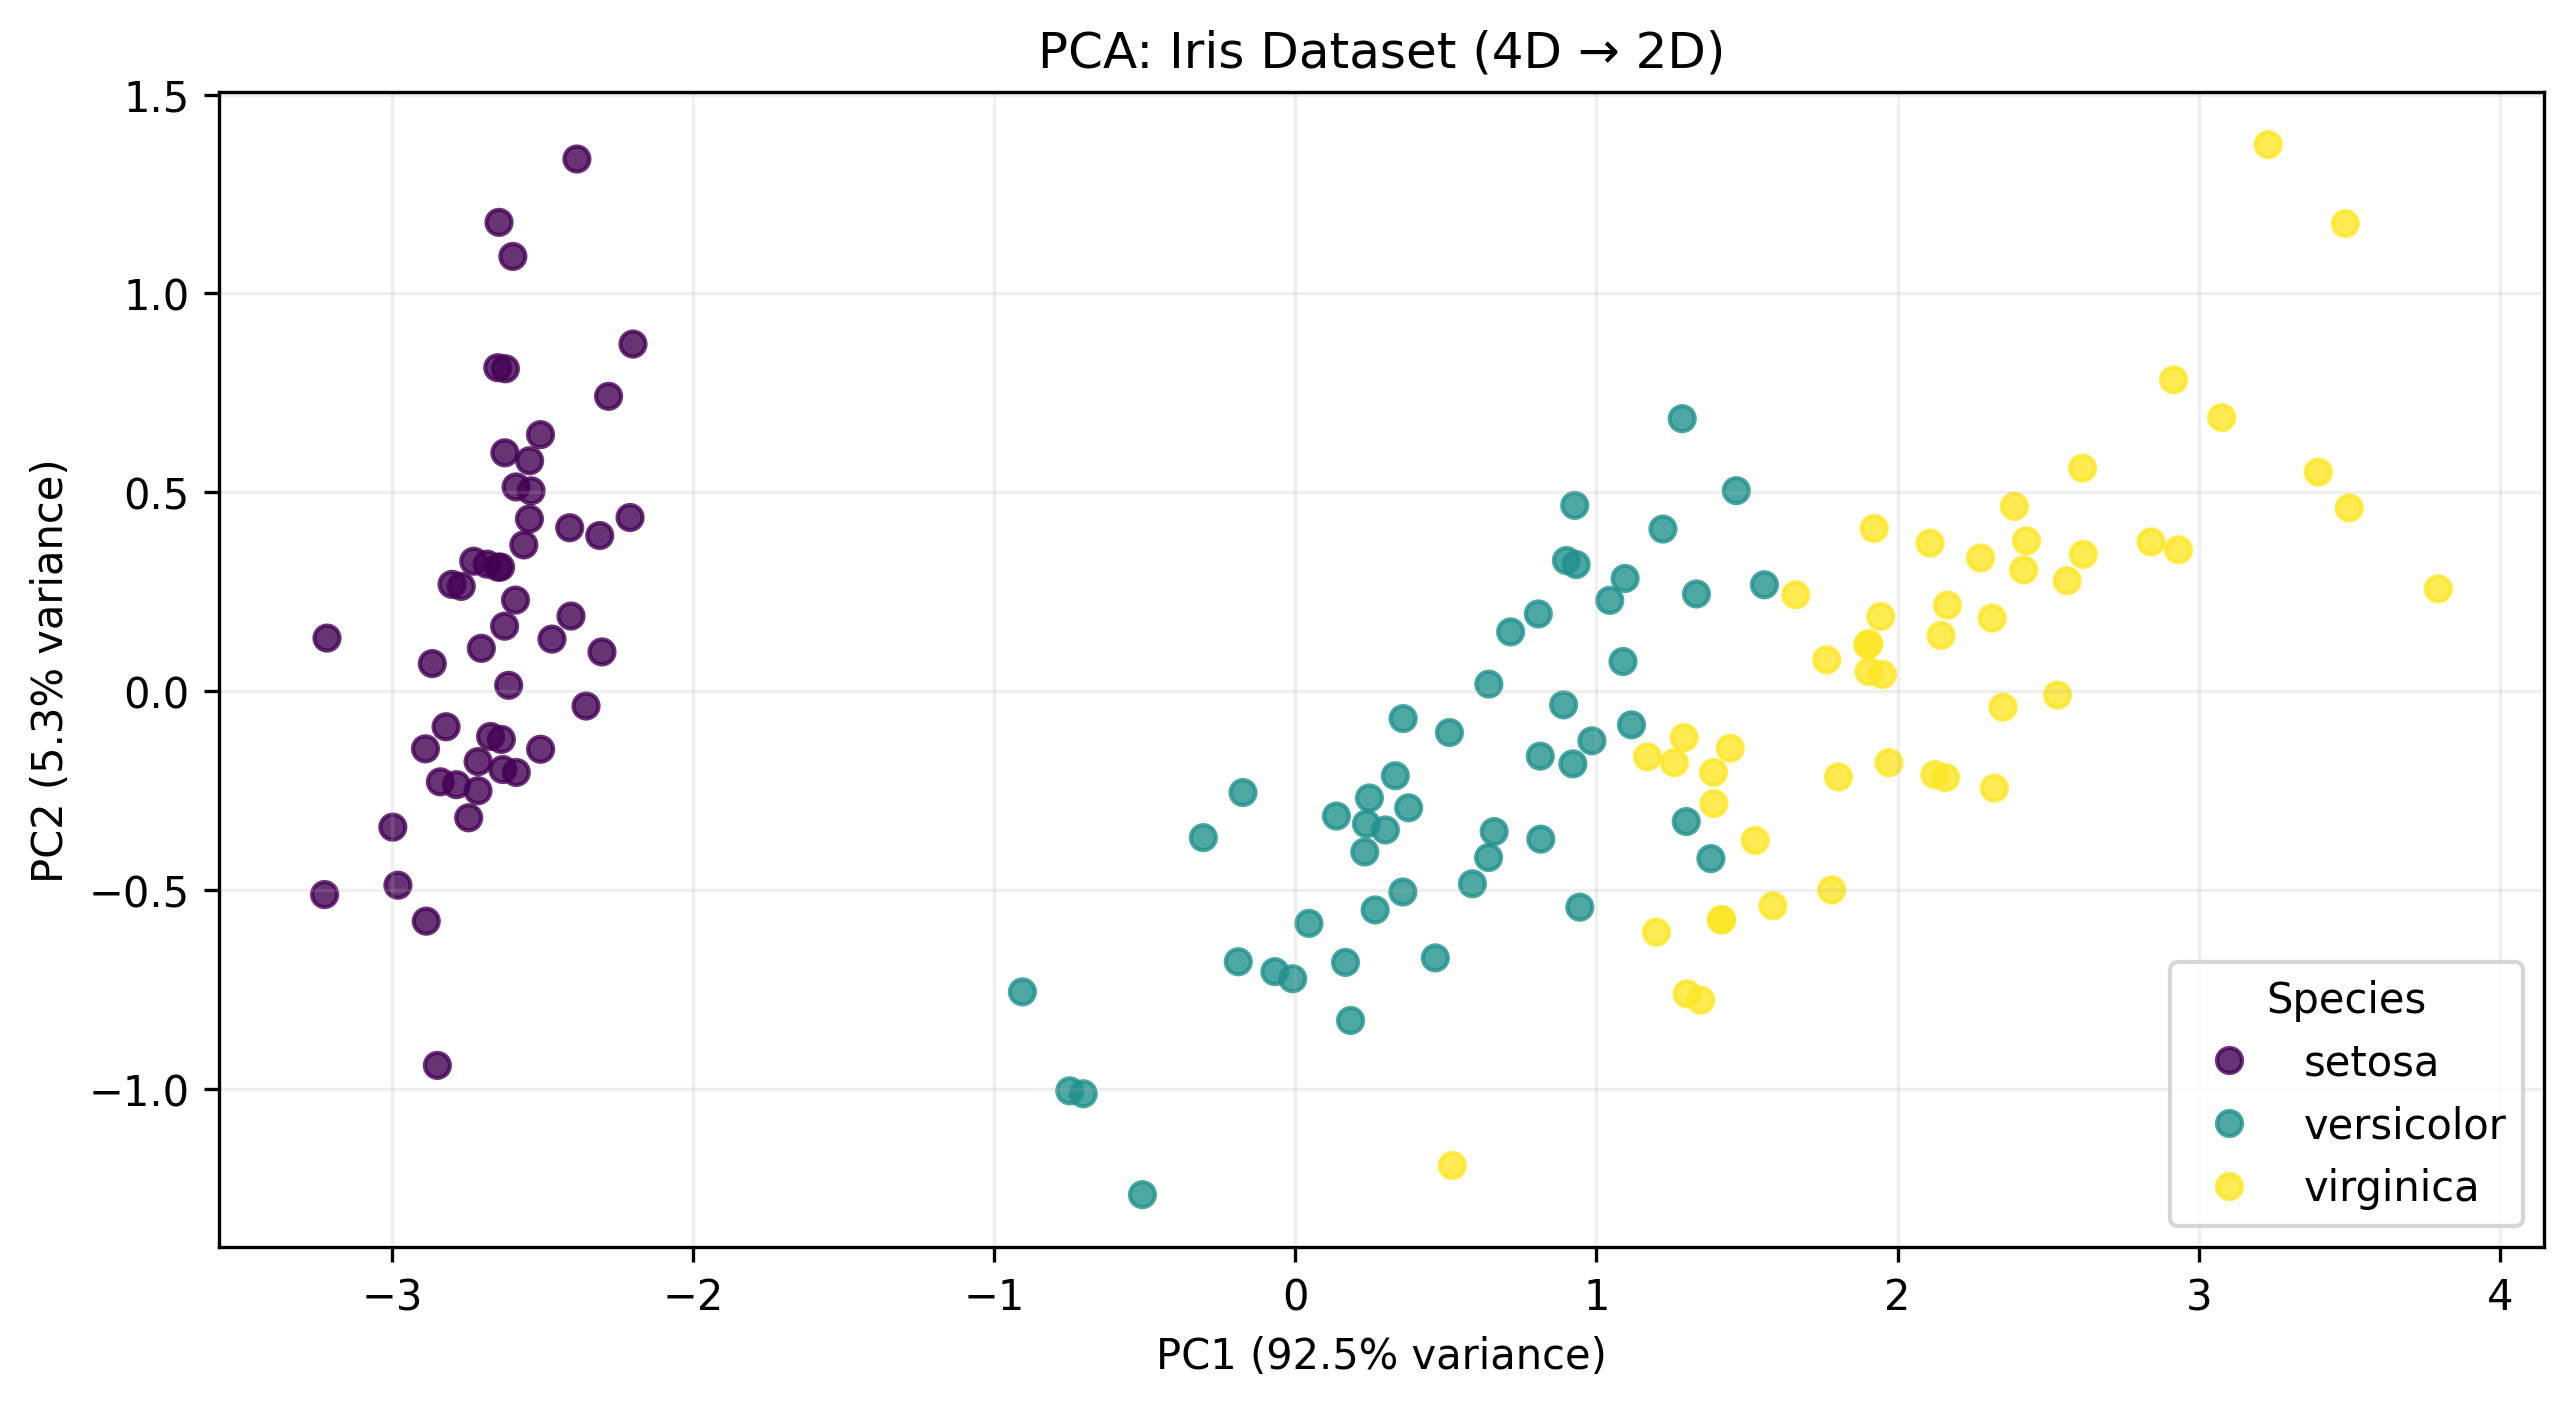
\includegraphics[width=0.65\linewidth]{images/pca/4D_to_2D.png} \\
    \end{center}

    \begin{itemize}
        \item We can visualize higher order data in 2 dimensions for EDA by projecting it onto PC1 and PC2.
        \item From data in PC1 and PC2 (92.5\% + 5.3\%) variance, we infer:
        \begin{enumerate}
            \item \checkmark \ Classification of \textbf{setosa} vs others is easy — clear separation. 
            \item \checkmark \ Classification between \textbf{versicolor} and \textbf{virginica} is harder due to overlap.
        \end{enumerate}
    \end{itemize}
\end{frame}


\begin{frame}{Individual Principal Component Analysis}
    \begin{center}
        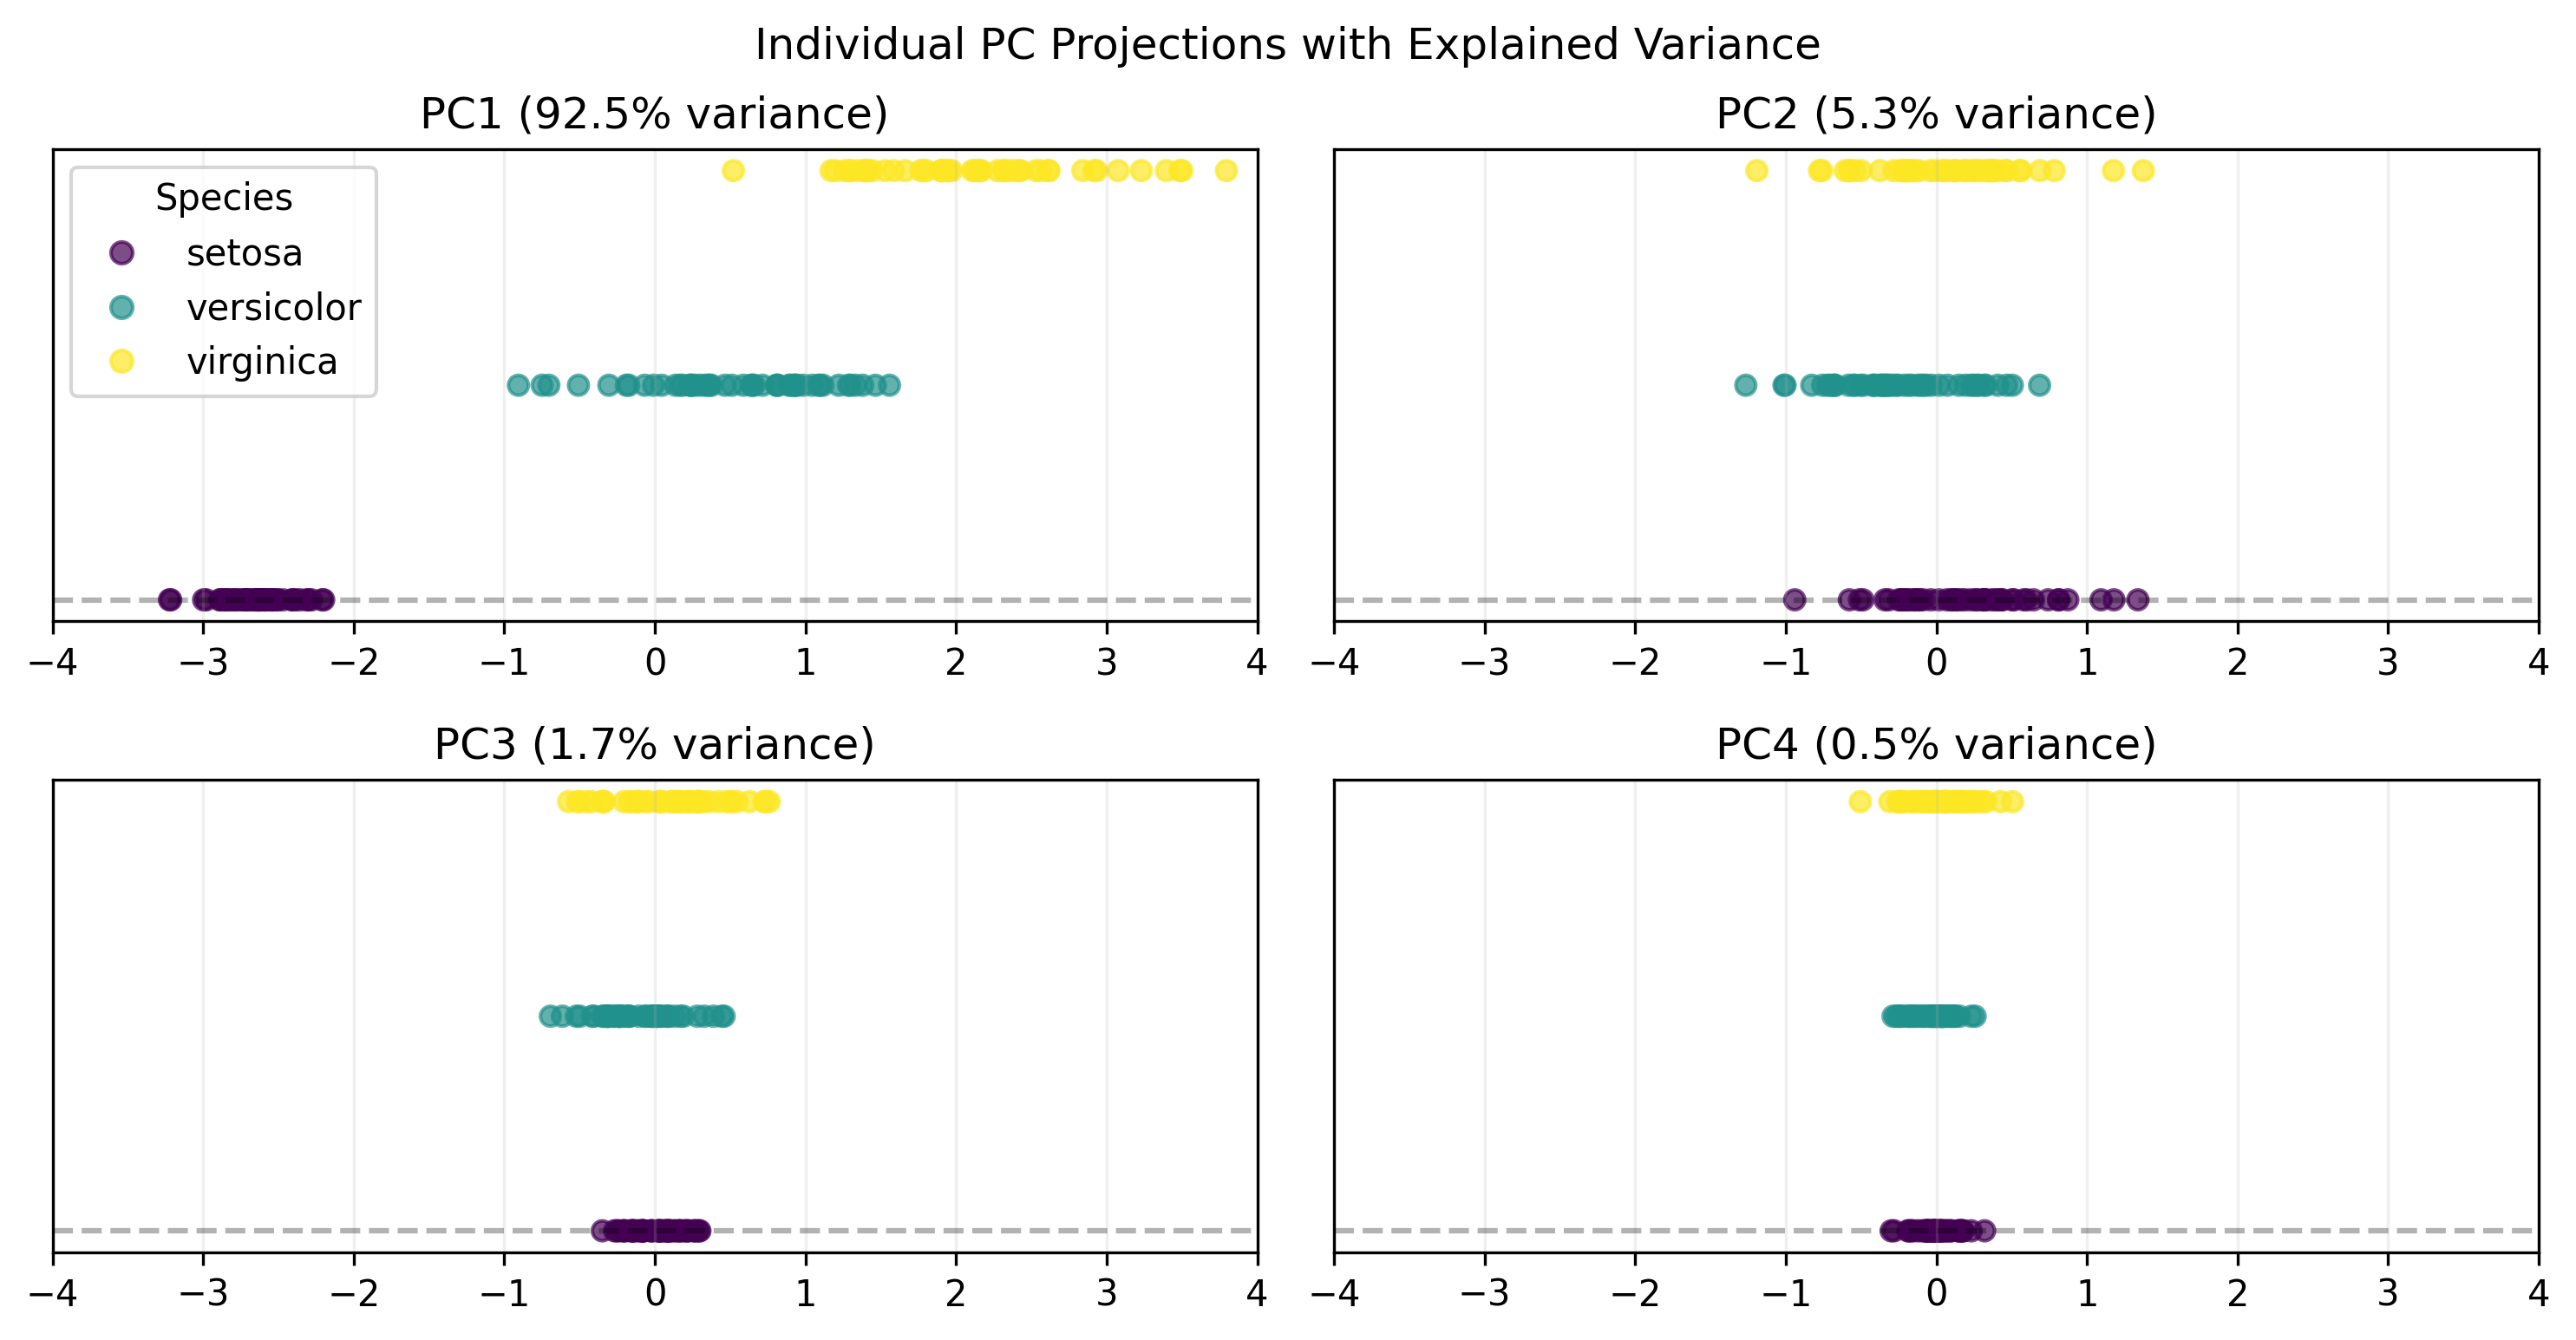
\includegraphics[width=0.8\linewidth]{images/pca/components.png} \\
    \end{center}

    We can see from the above plot, that only PC1 contains most of the information that is needed for classification. One can reduce the storage from $\mathcal{O}(n^4)$ to $\mathcal{O}(n)$, and still can (with significant confidence) classify the data into the three classes. 
\end{frame}



\begin{frame}{Dimensionality Reduction}
     \begin{center}
        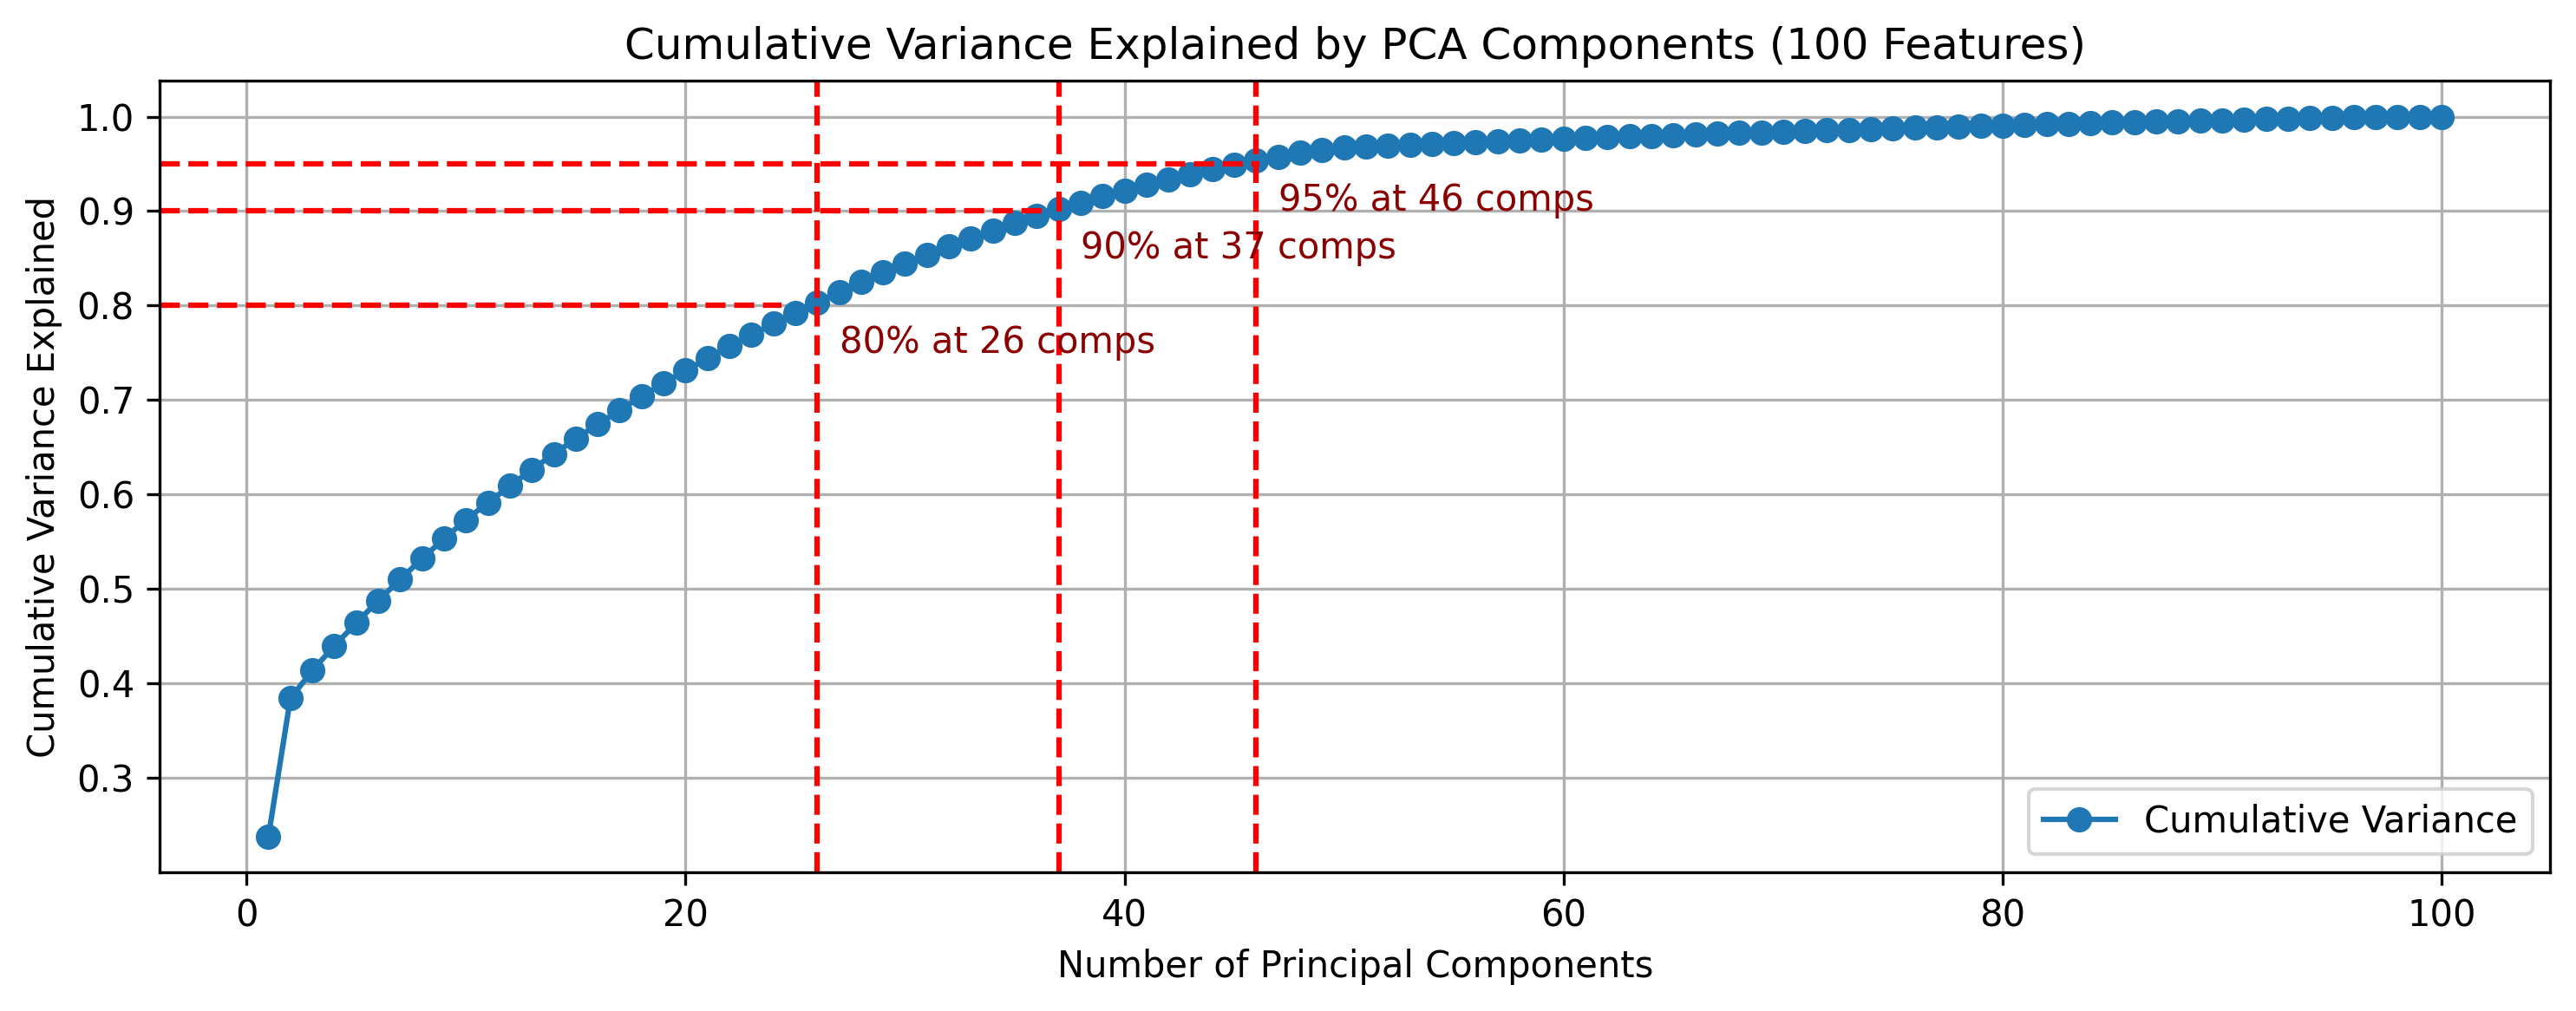
\includegraphics[width=0.8\linewidth]{images/pca/cumulative_variance.png} \\
    \end{center}

    \small{
        From the plot above, we observe the number of components required to capture various levels of variance:
    
        \begin{itemize}
            \item \textbf{80\% variance}: 26 components (26\% of original storage)
            \item \textbf{90\% variance}: 37 components (37\% of original storage)
            \item \textbf{95\% variance}: 46 components (46\% of original storage)
        \end{itemize}
        
        This highlights the efficiency of PCA in reducing dimensionality. Even at 95\% variance retention, we can reduce the dataset to less than half its original size while preserving most of the information.
    }
    
\end{frame}


\begin{frame}
  You can play around with the code and explore the examples presented in the previous slides by applying them to different datasets—whether your own personal datasets or other datasets available in scikit-learn—by using the following GitHub link:\\
    \vspace{1cm}
  \url{https://github.com/pesricha/MLDS-REVAMP/blob/main/notebooks/pca.ipynb}
\end{frame}



% END EXAMPLES

\begin{frame}{}
    \LARGE \centering \textbf{Thank You}
\end{frame}

\end{document}
